\section{Practical Considerations}
\label{section:implementation}

In this section, we discuss a few practical issues that we had to address as we
built \tool.

\myparagraphnodot{Where to Generate Test Cases?} 
%
The first practical consideration that we addressed was the question of which
platform to use to execute our test generator. One possibility was to use
Windows Phone, Xamarin's home platform. This requires us to execute \tool\
directly on a device or emulator running Windows Phone. However, we found that
the environment on such devices and emulators was somewhat awkward to use
during active development of \tool, \eg~to debug any issues that arose. We
therefore decided to develop and execute \tool\ on a desktop version of Windows
(8.1). Our hypothesis was that the desktop and phone versions would be largely
similar because they use the same \code{.NET} code base, and as a result, we
could use the desktop to generate the test cases and execute them as apps on
Windows Phone and Android devices.

This approach eased development of \tool, and for the most part our hypothesis
about the equivalence of the desktop and phone version of Windows was correct.
However, we found (and reported to Microsoft) 
%\cite{nader:connect:1} 
a case where the desktop and phone versions diverged in their semantics. In
particular, the public property \code{CurrencyDecimalDigits} of the class
\code{System.Globalization.NumberFormatInfo} is required to be a read-only
field according to MSDN documentation. While the read-only property holds in
the desktop version, the property is mutable in the Windows Phone version. We
also found, using differential testing against Android, a case where both the
desktop and phone version of Windows incorrectly implement the documented
semantics for a given property, while Android's implementation followed
Microsoft's documentation. In particular, the property \code{WebName} of
\code{System.Text.Encoding.BigEndianUnicode} must have the value
\code{UTF-FFFE} according to Microsoft's documentation, but the desktop and
phone version of Windows return \code{UTF-16BE}.

\myparagraph{PCLs and Test Generation}
%
A second issue that we had to address was the integration of \tool's test
generator and PCLs.  As previously discussed, \tool's test generator produces
test cases for a given input set of classes. It uses reflection to identify
public methods from those classes, the data types of their arguments and the
other properties of these classes, and uses this information in its test
generation algorithm.

However, PCLs pose a unique problem when used with \tool's test generator.
Recall that PCLs define the interface against which developers can build their
applications without concerning themselves with cross-platform portability
issues. PCLs enable this feature by transparently acting as forwarders---they
route calls from the application layer to the corresponding library in the
platform on which the application is loaded. Thus, PCLs usually do not contain
any of the executable code of the classes for which they act as an interface,
and merely contain forwarding stub code. As a result of this feature, when
\tool's test generator is provided with a set of PCL classes as input, it is
unable to use reflection to fetch the complete set of public methods, data
types and properties of the classes for which the PCL acts as a forwarder.

To address this issue, we had to extract the information required by \tool's
test generator by loading PCLs in a non-executable \textit{reflection-only}
mode. In this mode, PCLs are not executable, but can be queried using
reflection and return metadata by accessing the corresponding classes on the
platform. We then re-load the PCLs in executable mode, and use the metadata to
iteratively generate and execute test cases.

\myparagraphnodot{How to Package Test Cases?} 
%
Finally, we also had to address the issue of how to package up the test cases
for execution on the Windows Phone and Android platforms. Each test case is
packaged as a separate class that can be instantiated and executed. As
discussed above, we run the iterative test generation algorithm on the desktop
version of Windows. As a result, we have all the test cases available for batch
execution on the mobile platforms. 

\begin{figure}[t!]
\centering
\begin{tabular}{cc}
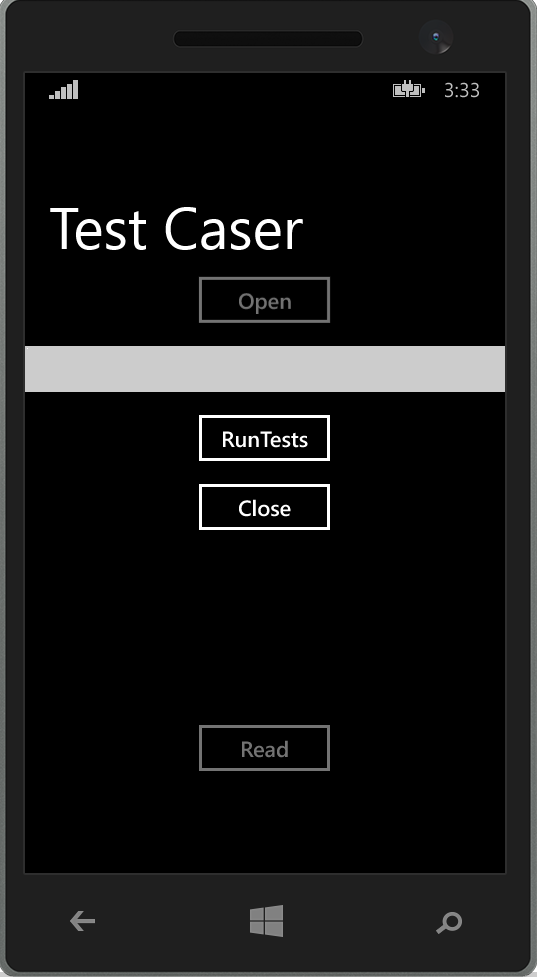
\includegraphics[keepaspectratio=true,height=5cm]{figures/windows.png} &
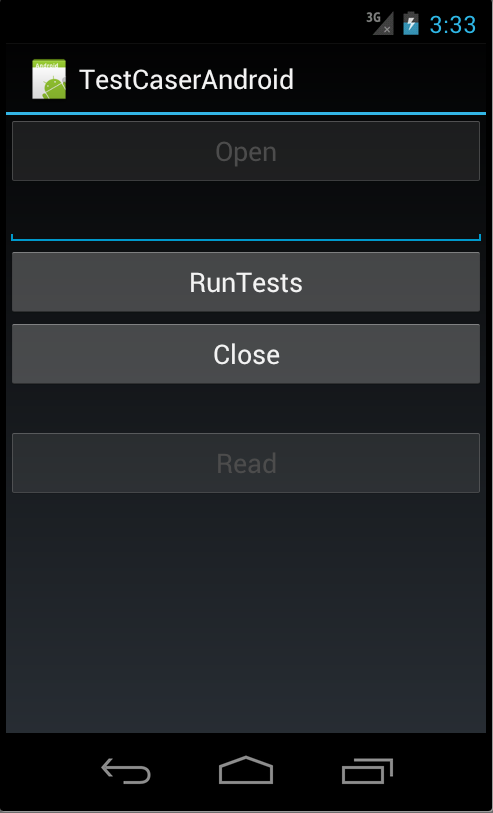
\includegraphics[keepaspectratio=true,height=5cm]{figures/android.png}\\
{\bf \small (a) Windows Phone version} &
{\bf \small (b) Android version}
\end{tabular}
\mycaption{Screenshots showing the UIs of the test case apps on Windows Phone
and Android.}{\label{figure:screenshot-testcase}}
\end{figure}

We package all the test cases into a single app each for execution on the two
mobile platforms. Both Windows Phone and Android require apps to define a UI.
We wrote this UI and the code to interface with the file system (to store the
logs generated when test cases are executed) within a  platform-specific
presentation layer, and packaged up the test cases as platform independent code
to be cross-compiled by Visual Studio and Xamarin. All the test cases generated
by \tool\ can be invoked at the press of a single button on the app.
\figref{figure:screenshot-testcase} shows the UIs of the Windows Phone and
Android versions of these apps. The UIs of these apps look rather
different---each app uses buttons and icons unique to the corresponding mobile
platform. However, because our test cases focus only on the
platform-independent PCL classes, the differences in the UI state do not
manifest as divergent state (and therefore as inconsistencies) during the
execution of the test-cases.

